%!TEX root = ttc14-fixml.tex

\section{Meta-Models}
\label{sec:MetaModels}

\enlargethispage{20mm}

\subsection{XML Meta-Model}

The XML model specified in the case study description~\cite{Lano2014}.

\begin{figure}[h!bt]
  \centering
  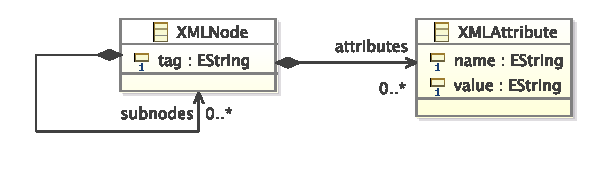
\includegraphics[width=.6\textwidth]{figures/XMLMetaModel.pdf}
  \caption{XML meta-model}
  \label{fig:XMLMetaModel}
\end{figure}

\subsection{ObjLang Meta-Model}

The meta-model representing an object oriented language originating from the Featherweight Java model~\cite{Igarashi2001} (concretely from the version available at the EMFtext website\footnote{\url{http://www.emftext.org/index.php/EMFText_Concrete_Syntax_Zoo_Featherweight_Java}}).

\begin{figure}[h!bt]
  \centering
  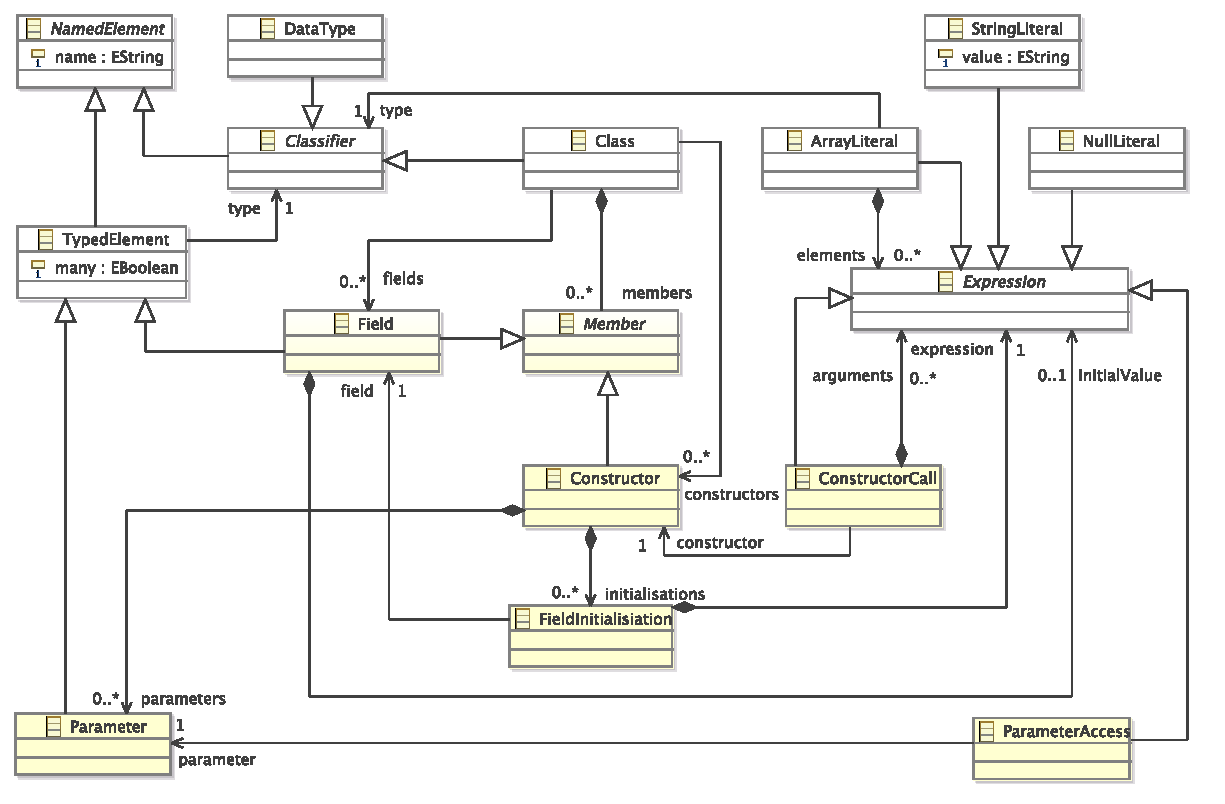
\includegraphics[width=\textwidth]{figures/ObjLangMetaModel.pdf}
  \caption{ObjLang meta-model}
  \label{fig:ObjLangMetaModel}
\end{figure}

